\documentclass{article} % For LaTeX2e
% We will use NIPS submission format
\usepackage{nips13submit_e,times}
% for hyperlinks
\usepackage{hyperref}
\usepackage{url}
% For figures
\usepackage{graphicx} 
\usepackage{subfigure} 
% math packages
\usepackage{amsmath}
\usepackage{amsfonts}
\usepackage{amsopn}
\usepackage{ifthen}
\usepackage{natbib}

\usepackage{caption}

\title{Project-II by Group MexicoCity}

\author{
Kevin Serrano\\EPFL\\
\texttt{kevin.serrano@epfl.ch} \And Youssef El Baba\\EPFL\\
\texttt{youssef.baba@epfl.ch} \And Alexandre Helfre\\EPFL\\
\texttt{alexandre.helfre@epfl.ch}
}

% The \author macro works with any number of authors. There are two commands
% used to separate the names and addresses of multiple authors: \And and \AND.
%
% Using \And between authors leaves it to \LaTeX{} to determine where to break
% the lines. Using \AND forces a linebreak at that point. So, if \LaTeX{}
% puts 3 of 4 authors names on the first line, and the last on the second
% line, try using \AND instead of \And before the third author name.

\nipsfinalcopy 

\begin{document}

\maketitle

\begin{abstract}
In this project we are given two problems: that of predicting the music listening counts for a given set of users based on their previous listening behaviour and friendship relations; and that of recognizing the presence of people in images. This report discusses preliminary observations on the given training data, and then results of testing various ML methods for prediction / classification.
\end{abstract}

\section{Exploratory Data analysis}
\label{sec:datadescr}
For the person detection dataset, there are 8545 images and a feature vector of dimensionality 9360 for each. The images are 3-channel (RGB) images, and the features are simply a vectorized form the image HOG features. Clearly this is a fat data matrix, even more so if we are going to split it into train/test datasets. Anyway, considering the huge number D, we are tempted to do some sort dimensionality reduction if we are to avoid extremely complex models and overfitting. This hints to the possibility of using PCA for this dataset. Or alternatively we can use neural networks, with the help of the Deep Learning Toolbox (kindly indicated by the course staff). We can also try using simple tools like $k-$means with $K = 2$ or SVM.

On initial visual inspection of the images and their corresponding features, it does seem that the HOG features for images with people are of a somewhat different nature. The various blocks containing the $(W \cdot W)$ feature blocks seem to have a much more varied orientation than for the images without people.

As to the music recommendation dataset, there are a total of 1774 users and 15082 artists. Each pair of (user, artist) is a data element, and the corresponding listening count number is the data.. If we change our convention to pairs of (user, user) we get another feature vector of size D=1 that is the friendship relation (currently given as a binary number, indicating a friendship existance). The format of the data set is peculiar with respect to usual matrices containing N rows of D columns (features) each. We can see that some users listen practically solely for a single artist with a high count when inspecting the provided $Y_{\text{train}}$ matrix.

On a different note, it seems daunting at first to predict specific count numbers for each (user,artist) pair, as usually the recommendation in such systems are the k most “likeable” artists for a specific user. One way to go is to predict, using a computed probability for each (user, artist), a sort of score that is, a count that will be simply the maximum number of counts of the user when the score is 1, and adjusted linearly with the score as the coefficient.

\section{People Detection}
\subsection{Neural Networks}
When playing with the person detection code given to us, using the deep learning toolbox, the training error obtained was 0.745, which is approx. 75%, not bad at all for a first trial. Since the number of data points is small, a non-zero value of the dropout rate might help. We should also consider L2 penalization (similar to lambda used in ridge regression) in the late stages of the project to reduce the effects of overfitting. We will then try to measure the average test TPR with k-fold cross-validation.

Continuing with neural networks testing, we tried adding a dropout fraction of 0.3 and see if it could improve the error rates. The stable (after 25 epochs) mean-square error (obtained using the native plot of the Deep Learning Toolbox nntrain function) for the methods without and then with dropout was 0.005774 and 0.006937 respectively. Oddly enough though, average TPRs for these methods are 0.75 and 0.787 respectively. A second run with another seed for the Matlab random number generator gave other final MSEs and TPRs, this is because NN are very sensitive to the initial seed. So the seed for all further trials was manually set to 8339 (given by the course staff) . Adding a dropout seems to enhance our TPR,, but gains are somewhat mitigated for bigger FPRs. The batchsize for these methods (a parameter in the Deep Learning toolbox) was also tampered with, when we tried to take the whole training/data as a batch (batch size ~4272), however this turned out to be a bad idea as the convergence of the MSE cost (on the toolbox’s training graphs) only attained 0.014 at the lowest level, much higher than with a batchsize of 100. Then we tried changing the internal activation functions from tanh to sigmoids, with an improvement of the MSE / TPR to 0.002975 and 0.795, which was quite remarkable. The last 2 variants to be tried were simple NN with $L_2$ weight penalty equal to 1/1000 and simple NN with both sigmoid activations and a dropout of 0.3, which respectively gave MSE / TPR values 0.006758 / 0.772 of 0.00404 / 0.844. These results 

In addition to that, logistic regression was given a try, and it gave a TPR of 0.7521. Then Penalized logistic regression with a lambda of 1/50 also gave the same TPR. The $\lambda$ for the logistic regression clearly wasn’t adequate.

One clear conclusion that can be drawn here is that internal sigmoid activation functions, instead of tanh, help a lot. They are going to be used for the final model then (if using NN).

Clearly, each of these additions to the basic NN model improves things, on its own, a bit. However when they are applied together, things improve considerably (as indicated by the last cited and quite high TPRs). Of course, the values for these parameters (dropout and $L_2$ penalty) were chosen arbitrarily. Similarly, Penalized Logistic regression can have a different optimal lambda, which should be cross-validated, and might result in higher TPR. 

We cross-validated parameters for the NN: namely the dropout, $L_2$ weight and dimension (depth mostly). Following are the corresponding plots, respectively. We can see that a dropout value of 0.43 is actually the best one to choose (the one with minimal test error, red curve) This was done for 15 values of the dropout, $k=4$, and 15 different seeds. We then cross-validated the $L_2$ weight penalty parameter for NN and obtained an optimal TPR of 81.45\% for a weight penalty of $10^{-6}$ (while setting the dropout to a static value of 0.43). We used 15 seeds and 20 values of the $L_2$ weight, with $k = 4$.

A last thing we wanted to cross validate was the depth, but due to time restrictions and a huge computational workload for doing so (for a high number of units in profound NNs), we simply decided to pick dimensions based on a try out of various ones by hand.
\begin{figure}
\centering     %%% not \center
\subfigure[NN with various dropouts]{\label{fig:nnkcvdrop}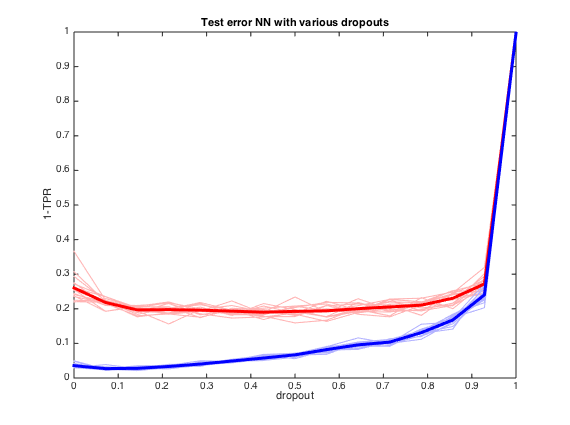
\includegraphics[width=0.49\textwidth]{images/NNKCVplotdropout.png}}
\subfigure[NN with various L2 weight penalties]{\label{fig:nnkcvl2}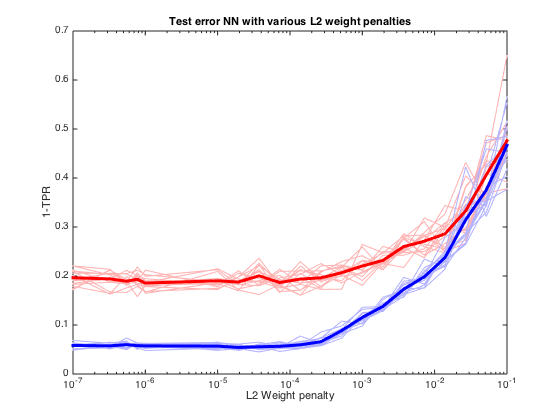
\includegraphics[width=0.49\textwidth]{images/NNKCVplotL2weight.png}}
\caption{Parameter cross-validation for neural networks}
\end{figure}

\subsection{Penalize Logistic regression (cross-validation for $\lambda$)}
Penalized logistic regression was cross-validated (for the lambda parameter) to see which setting gives the best estimated TPR. The error metric taken was 1-TPR, which made simple sense. $\lambda$ values between $10^{-3}$ and $10^2$ were tested, 15 of them, and using 15 different seeds. So a total of $15 \cdot 15=225$ gradient descent runs for PLR were tried, giving the following plot (Figure \ref{fig:TEPLR})
It seems that, roughly, the more we increase lambda, the better our test error equivalent (1-TPR, which is actually the False Negative Rate) is.
\begin{figure}[h!]
\centering
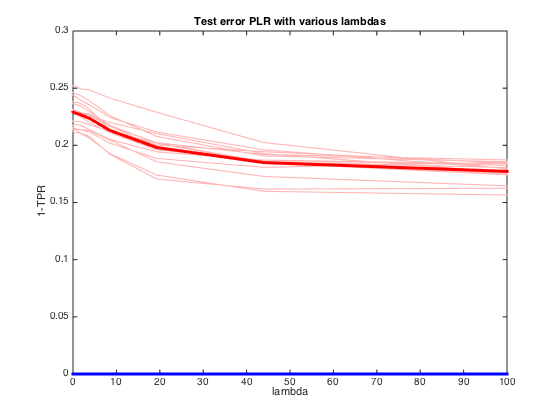
\includegraphics[scale=0.6]{images/PLRKCVplot.png}
\caption{Test error PLR with various $\lambda$}
\label{fig:TEPLR}
\end{figure} For $\lambda$ = 44, we deem it the test error no longer decreases significantly and it’s sufficiently good at 0.1849 (this corresponds to a TPR of 0.8151). This would be the best possible variant in the Logistic regression family to use. It remains to be seen at this point, however, if other ML methods can do better, especially after all their variants have been cross-validated (NN with various dropouts and $L_2$ weight penalties for instance). (red curves show the 1-TPR for test set, using model trained on a different training set, for each lambda, each curve being the result of a different seed, the bold curve being the average).

\subsection{$K-$means}
We then tried using $k-$means on the same train and test sets used for the previous methods, with identical normalization (essentially how the provided demo script did the split). The MATLAB $K-$means is particular in the sense that it does not take the actual (true) labels (person / no person) of each point (image) in account when computing its assignment, it simply renames the classes as $1, 2, 3, \cdots, K$. What it does is it simply clusters in a best effort manner the points, and assigns random labels to them. We tried at first to simply compute the MATLAB labels on the test data and reassign them to $-1$ and 1, which gave a TPR of 0.0057 (or 0.57 \%), very low for any practical purpose to say the least. We then tried to re-wrap the $k-$means function in another one generating a "model" (centroids + labels of the centroids computed as the mean of the labels of their assigned points) which now uses the true labels of the points. And another function which, as is typical of other methods, predicts the assignments of new points (using euclidean distance to centroids). This now resembled classical model based methods, however it also failed miserably with a TPR of $5.8*10^{-4}$. This can be explained by the fact that the cluster of no-person images is much, much larger than the one with person-containing images, hence when assigning the labels to the cluster means they consistently get the label "no-person" making the result a static label $-1$. As taking the mean label of the cluster points and assigning it to the cluster mean is an integral part of the $K-$means algorithm, this ML method is probably not the one to use here.

\subsection{Support Vector Machine}
The next method we tried to apply on the people detection dataset was SVM. We used the \texttt{fitcsvm} and \texttt{predict} functions of MATLAB, to be able to obtain posteriors probabilities and not just hard assignments. We tested plain old SVM, with a linear kernel, and by taking a slight transform of the posterior we were able to obtain a TPR of 80.59 \%. We tried varying the $C$ constant parameter, trying values of 0.1, 0.5, 2 and 5, however they all gave the same TPR. We then tried using an RBF kernel, with $\sigma$ values of 0.5, 1 and 2, but they all gave a very low, consistent TPR of 0.0582 \%. This is very similar to what we get by simply predicting a $-1$ (no-person) for all the images. The prospects for the basic variant of this method provided good performance, but its lack of flexibility for further improvement makes us believe we should opt for another ML method for this dataset instead.

We then launched several small cross-validation tests and determined that the best SVM variant was the one using the RBF kernel and a $\sigma$ of 81 (plots not shown here for brevity)

A comparison plot for fits using the staff-provided data split and seed, using the various methods, is given in Figure \ref{fig:pdplot}, using the same seed. It gives the test error equivalent (TPR) for each one.
\begin{figure}
\centering
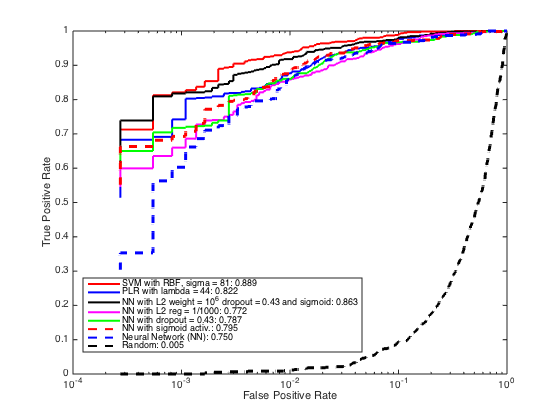
\includegraphics[width=1\textwidth]{images/PDTPRcomparisonplots.png}
\caption{Comparison of different methods for People detection}
\label{fig:pdplot}
\end{figure}
\section{Music recommendation}
\subsection{Histogram}
Following is a the histogram of the counts for the Music recommendation dataset (Figure \ref{fig:histC}). The max count is 352698, which is huge. Moreover the number of counts $>$ 5000 is rather small. That’s why we’re only showing the bins for the counts that are smaller or equal to 5000, the rest being generally present once or twice at most.

After observing the histogram of the counts, as proposed by the course staff, we can see that despite the high maximal count, most of the data is concentrated in the low-count range (1-3500). Going out on a limb here we might consider any count quite outside of this interval to be an outlier, however things are a bit nuanced: if we start removing outliers from the data (which is already sparse) we run into the problem of deciding how far the point has to be from this interval to consider it as such. That decision is very difficult to make, especially considering that music listening - as any human-  behaviour cannot be expected to always follow mathematical rules.

A second conjecture is that, inside this interval, most counts are still concentrated at the lowest range. It’s as if the histogram of the counts decays exponentially fast, which is why taking the logarithm (of the counts) would change the $x$ axis scaling in some sorts and produce a more bell shaped curve, i.e. a Gaussian. This is experimentally confirmed by taking the histogram of the counts (full counts, not restricted to the interval, see Figure \ref{fig:histC}) and then taking the histogram of the log of the counts, which does correspond to a Gaussian, as shown in Figure \ref{fig:loghist}. This shows potential for such a transform to be used before applying ML methods, especially those one imposing Gaussian-distributed restrictions on their data.
\begin{figure}
\centering     %%% not \center
\subfigure[Histogram of counts]{\label{fig:histC}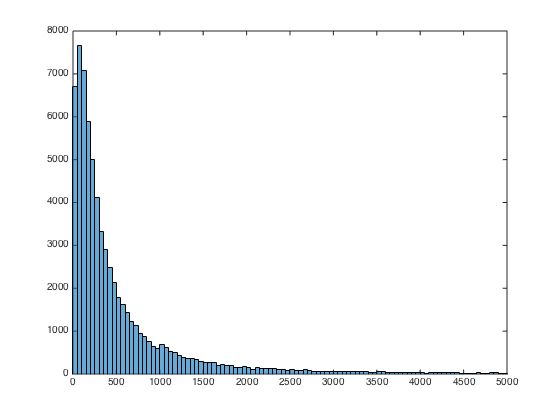
\includegraphics[width=0.49\textwidth]{images/countHist.png}}
\subfigure[Histogram of log transformed counts]{\label{fig:loghist}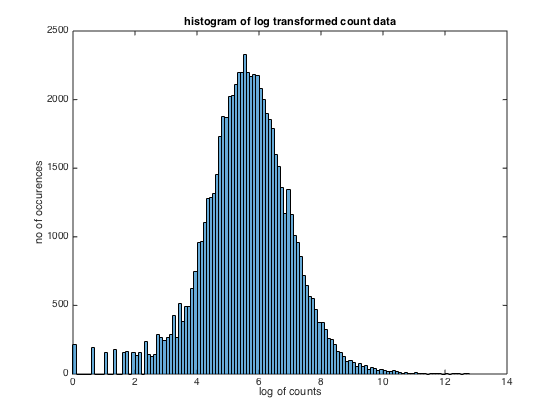
\includegraphics[width=0.49\textwidth]{images/MRhistlog.png}}
\caption{Histogram of count data for MR}
\end{figure}


\subsection{PCA/SVD}
We ran the PCA algorithm on the full-format $Y_{train}$ data. Nevertheless the ALS algo (PCA with the ALS option) does not work with this matrix, as it seems that $Y_{train}$ is a too large a matrix even if it is sparse in practice.

Therefore we applied the SVD decomposition on $Y_{train}$ to see if we can reduce in practice reduce the dimensionality of our problem. To illustrate that possibility, following is the plot (Figure \ref{fig:modk}) of the cumulative fraction of variance explained vs the modes. (For mode 1 we use singular value $s_1$ and its corresponding vector, for mode 2 we use $s_1$ and $s_2$ and their etc, increasing the rank of our approximation). The result can be summarized in that the 900 most significant vectors (highest singular value) explains 95\% of the data’s variance, which means they can be roughly sufficient to use as a basis for training ML models and predictions.
\begin{figure}
\centering
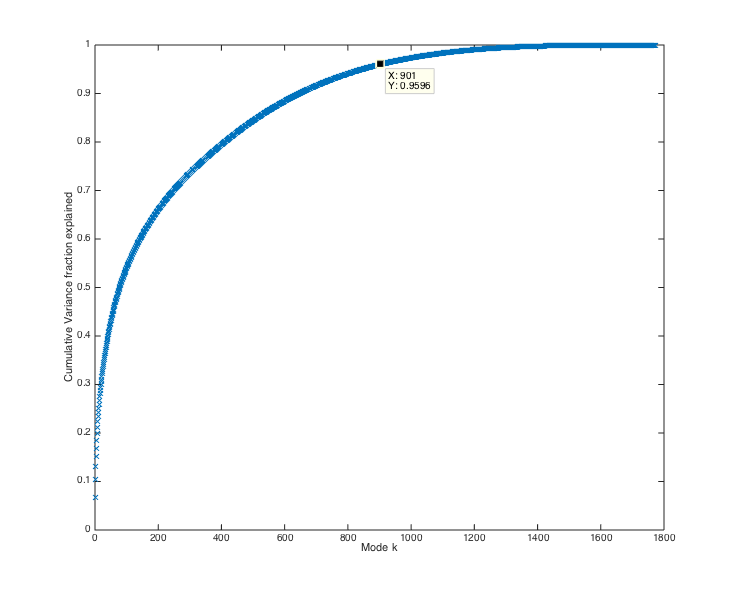
\includegraphics[width=1\textwidth]{images/svdvariancemodes.png}
\caption{Cumulative variance fraction explained}
\label{fig:modk}
\end{figure}

\subsection{Basic mean-based predictions}
One of the simplest prediction method is to use averages to predict. The first thing we have done is to compute the average listening per artist on our training set.  Then using only the positive values in our test set, we can compute the RMSE between our prediction and the real values. If we don’t apply any transformation to the data, we obtain a RMSE of 6400. We can see that this is quite a high number but nevertheless expected since the RMSE supposes an Gaussian input and that the average method is not a good one. 

Then we applied the log transformation to obtain a more Gaussian input as seen in Figure \ref{fig:loghist}. We then compute the RMSE based on the same principle as before and rescale the result with the exponential to obtain an RMSE of 4130 (8.3 in log scale), which is already much better.

\subsection{Collaborative-filtering}
Let $UA$ (users-artists) be equal to $Y_{train}$. We split the data into a training set $ua_{tr}$ and a test set $ua_{te}$. The values inside the matrix are the number of time an user heard an artist. One of the principle features of the problem now is to say whether a user “likes” an artist of not, and ideally to know how much.

We first tried to normalize each row independently so that we will get values between 0 and 1.  Then we applied the following method : We created the matrix $P$, which is a diagonal matrix where each value in the diagonal is the total listening count for each user, (there are problems with users with total count $= 0$, however those don’t exist in our dataset). Hence, this matrix is invertible.

Using this inverse we can compute the similarity matrix $S_u$ between users. At this point we don’t take into account the social graph, but it looks promising to refer later (if we can assume that friends are more likely to like the same artists). The similarity matrix $S_u$ should contain 1 in the diagonal ( a user is maximally similar to himself). However this is not the case in our dataset : when we computed the similarity of the user using the formula $ua_{tr}\cdot ua_{tr}^T$ then we obtain the total number of listening in common with other users. That means to get a diagonal of $1$’s, the matrix $P$ should be defined differently : instead of having a diagonal matrix where each entry is  total listening count of user $i$, we should simply have the same values as $ua_{tr} \cdot ua_{tr}^T$ in the diagonal matrix $P$ and $0$ elsewhere. Then we will measure the cosine similarity between another user. Note that this is possible to do without normalizing the data, as we obtain the same results regardless. Computing the average of listing by users $u_a$ and multiply this with the scores obtained from the similarity matrix ($S_c = S_u \cdot ua_{tr}$). After playing with numbers, we discovered that we can predict the counts $P_r = (X\cdot u_a)^{0.8}$ where $P_r$ is the predictions. When we compare this prediction with the test set $ua_{te}$, we obtain a rmse of $3.06$ in log scale, which is quite accurate. This is the weak prediction.

One idea is to use the social graph along with the similarity matrix we obtained is to see if it is indeed the case that friends are similar users ( listeners), but not the other way around. Therefore, when we want to add a new users and predict his counts (taste in music), one possibility would be to use the information in the social graph and then use the similarity matrix to predict

So finding the social relation between users requires finding the position of $1$s in the social graph. With these positions we can check what is the similarity between friends and compute the average similarity. We obtained experimentally an average of $0.2145$, which means their taste are not as correlated as we thought, putting the usefulness of the social graph into question again. We can use this number when we want to predict counts for a new user: we can look into the social graph to obtain the relationship between the new user and all existing users and then decide on their similarity between them. This similarity for new user $i$ is computed as the mean similarity of all his friends in the known set ($Y_{train}$) for a particular user $j$. We obtain a new similarity matrix and can compute the predictions. Basically this is the same idea as before but only using friends of the new users.
\subsubsection{Recommendations}
Using the similarity matrix $S_u$ and the dataset, we computed $S_c = S_u \cdot UA$ as before to obtained the scores. With these scores we can recommend artists to existing users. For example in Figure \ref{fig:rec}, using the first user in the dataset, we see his top-5 listening and the top-5 recommendations. The method to compute this recommendation is called user-user collaborative-filtering.
\begin{figure}[h!]
\centering     %%% not \center
\subfigure[Top-5]{\begin{tabular}{c|c|}
 & User 1\\
 \hline
1 & Morrissey\\
2 & The Smiths\\
3 & Elvis Presley\\
4 & The Housemartins \\
5 & Blur\\
\hline
\end{tabular}}
\subfigure[Top-5 recommendations]{\begin{tabular}{c|c|}
 & User 1\\
 \hline
1 & Just Surrender\\
2 & Huun-Huur-Tu\\
3 & Beverly Kenney\\
4 & Imperative Reaction \\
5 & Maze featuring Frankie Beverly\\
\hline
\end{tabular}}

\caption{Top-5 recommendation for user 1}
\label{fig:rec}
\end{figure}

\section{Summary}
For people detection, we decided to opt for NN with the cross-validated parameters instead of the otherwise best-TPR simple SVM method. That is because we found the output of NN predictions to be more stable than that of SVM (score between -1 and 1, in contrast to usually off-interval output for SVM). The final parameters used are $L_2$ weight = $10^{-6}$, a dropout of 0.43 and dimensions of $[D \ 250 \ 50 \ 10 \  2]$, and using sigmood internally, we also increased the number of epochs to 40.\\

For the music recommender we managed to recommend songs successfully to existing users based on their similarity with other users. We predicted the counts using different models with sometimes good and very bad results. Our best was the model based on the similarity (collaborative-filtering) for the weak prediction. Some other model could have been tested if we had more time, for example clustering.
\subsubsection*{Acknowledgments}
We would like to thanks the teaching team for their availability during the exercise sessions and office hours but also on the forum. We also want to thanks Youssef who organized the milestone of the project.
\subsubsection*{References}
Kevin Murphy, Machine Learning : A Probabilistic Perspective {\em The MIT Press
Cambridge, Massachusetts
London, England,2012}\\
Trevor Hastie,Robert Tibshirani,Jerome Friedman : The Elements of
Statistical Learning. Data Mining,Inference,and Prediction. {\em Springer, 2008}\\
Gareth James,
Daniela Witten,
Trevor Hastie,
Robert Tibshirani:An Introduction to Statistical Learning.{\em Springer, 2013}
\end{document}
